\documentclass[unknownkeysallowed, 10pt, a4 paper, handout]{beamer}

% Custom beamer theme
\usepackage{../style/beamerthemeCustom}
\newcommand{\HRule}{\rule{\linewidth}{0.5mm}}   %FOR TITLEPAGE

\usepackage{changepage}       % adjustwidth

\setlength\parskip{0.3cm}

\newcommand{\focus}[1]{\textbf{\textcolor{red}{#1}}}
\newcommand{\ra}{$\longrightarrow$ }
\newcommand{\lra}{$\longleftrightarrow$ }

\newcommand{\code}[1]{\colorbox{black}{\color{green}\texttt{#1}}}

% Command to create two side-by-side minipages
\newcommand{\sidebyside}[5]{
  \begin{minipage}{#1\textwidth}
    #2
  \end{minipage} #3 \begin{minipage}{#4\textwidth}
    #5
  \end{minipage}
}

\begin{document}


\begin{frame}[label=outline]{Science with the Computer}
  You can do Science with a computer !
  \begin{columns}[T]
    \begin{column}{.53\textwidth}
      \begin{itemize}
        \item Text Editors and WYSIWYG programs for writing
        \item Tools and libraries for data handling and visualization
        \item Data acquisition and storage
        \item Modelling and numerical algorithms
      \end{itemize}
    \end{column}
    \hfill
    \begin{column}{.45\textwidth}
      \vspace{15pt}
      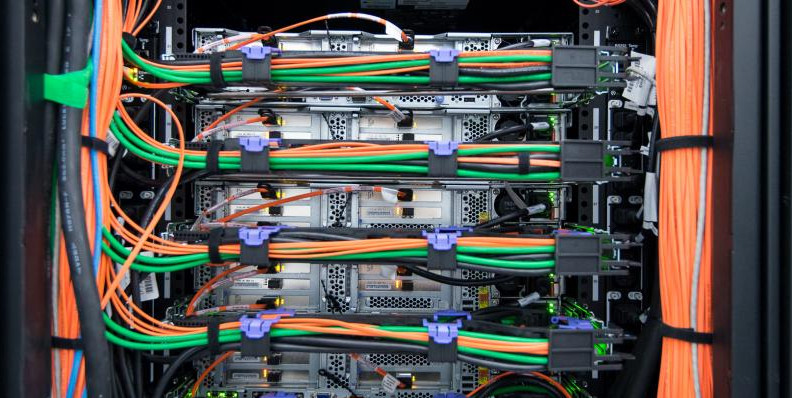
\includegraphics[scale=0.2]{pics/20140924103021_DSC_6759_MHPC.jpg}
    \end{column}
  \end{columns}
  It can get to such complexities that a whole new Science has emerged:
  \begin{center}
    \textcolor{red}{Computer Science} : 
             study of computers and computational systems
  \end{center}
\end{frame}


\begin{frame}[label=pipelining]{Writing your own program - 1}
  Use the building blocs of existing programs and create a complex
  \textcolor{red}{\textbf{pipeline}} of stages to reach the desired processing
  \begin{columns}[T]
    \begin{column}{.33\textwidth}
      \vspace{20pt}
      
\includegraphics[scale=0.25]{pics/plumbing-pipes.png}
    \end{column}
    \hfill
    \begin{column}{.66\textwidth}
      \begin{itemize}
        \item \textbf{Pros} : No programming in the general sense involved,
          just carefully examination of the input and output of existing
          system programs to create the required processing. The REAL UNIX way
          of using a computer.
        \item \textbf{Cons} : Limited by the possible processing allowed by
          system programs, generally related to text file manipulation,
          non portable across different systems
      \end{itemize}
    \end{column}
  \end{columns}
  Example:
  \begin{center}
    \code{ls -al | grep \${USER} | tr -s ' ' | cut -d " " -f 5 > sizes.txt}
  \end{center}
\end{frame}


\begin{frame}[label=scripting]{Writing your own program - 2}
  Use generic \textcolor{red}{\textbf{scripting language}} interpreters which
  can more flexibly allow runtime evaluation of a processing
  \begin{columns}[T]
    \begin{column}{.66\textwidth}
      \begin{itemize}
        \item \textbf{Pros} : More flexible, eventually the shell itself can be
          used, can use specialized libraries for compute intensive tasks,
          rapid prototyping
        \item \textbf{Cons} : Need to learn a programming language, not as
          fast as a system binary can be.
      \end{itemize}
    \end{column}
    \hfill
    \begin{column}{.33\textwidth}
      \vspace{10pt}
      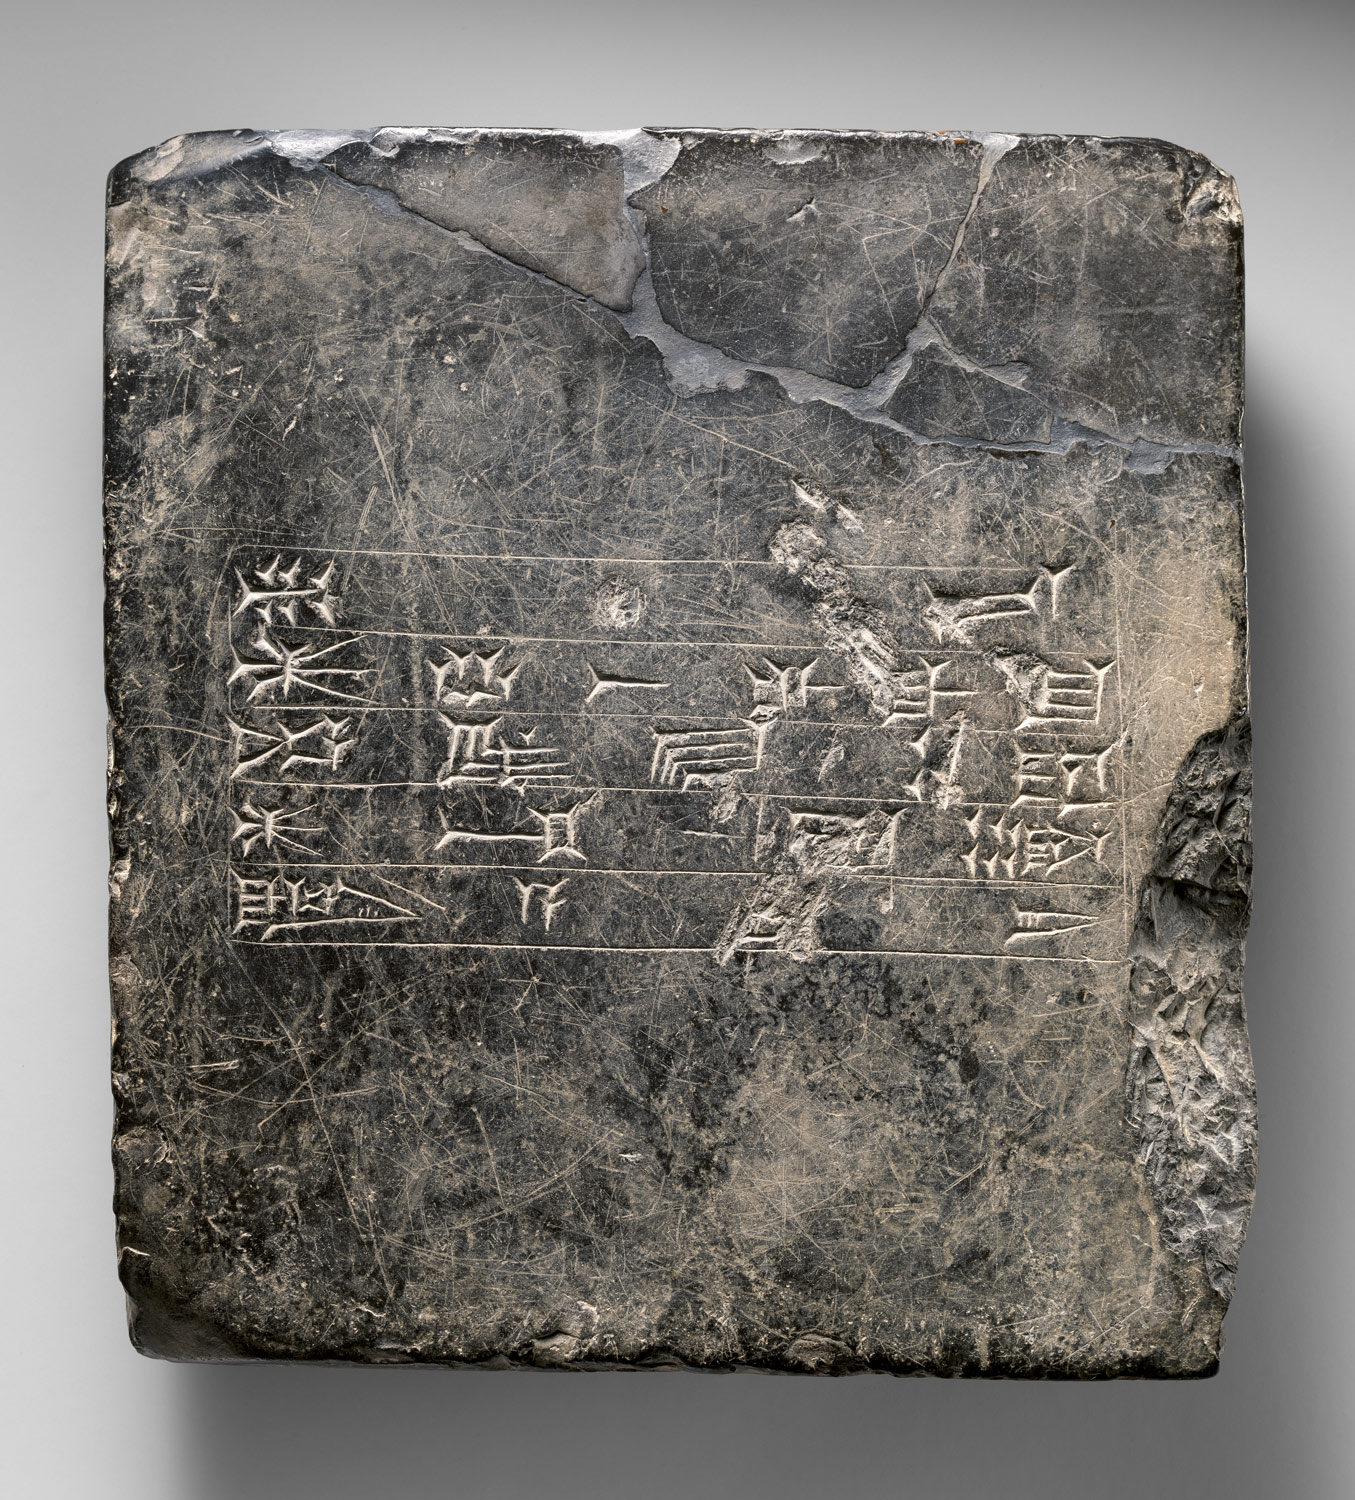
\includegraphics[scale=0.07]{pics/cuneiform.jpg}
    \end{column}
  \end{columns}
  Example:
  \begin{itemize}
    \item Shell scripting
    \item Python language
    \item R statistical language
  \end{itemize}
\end{frame}


\begin{frame}[label=compiled]{Writing your own program - 2}
  Use a low level \textcolor{red}{\textbf{programming language}} which is
  parsed by a program called \textit{compiler} to create a system binary
  program
  \begin{columns}[T]
    \begin{column}{.23\textwidth}
      
\includegraphics[scale=0.35]{pics/225px-ISO_C++_Logo.png}
    \end{column}
    \hfill
    \begin{column}{.76\textwidth}
      \begin{itemize}
        \item \textbf{Pros} : Fast execution time, tailored processing to the
          problem to solve
        \item \textbf{Cons} : Need to learn a programming language, not as
          flexible as a scripting language, may require writing code even
          for very simple and common tasks best approached by generic 
          system programs.
      \end{itemize}
    \end{column}
  \end{columns}
  Example:
  \begin{itemize}
    \item Fortran Programming Language
    \item C/C++ Programming Language
  \end{itemize}
\end{frame}


\begin{frame}[label=Fortran]{Fortran program}
  \begin{center}
  \Large{Fortran source files are text files}
  \end{center}
  \begin{columns}[T]
    \begin{column}{.23\textwidth}
      \vspace{30pt}
      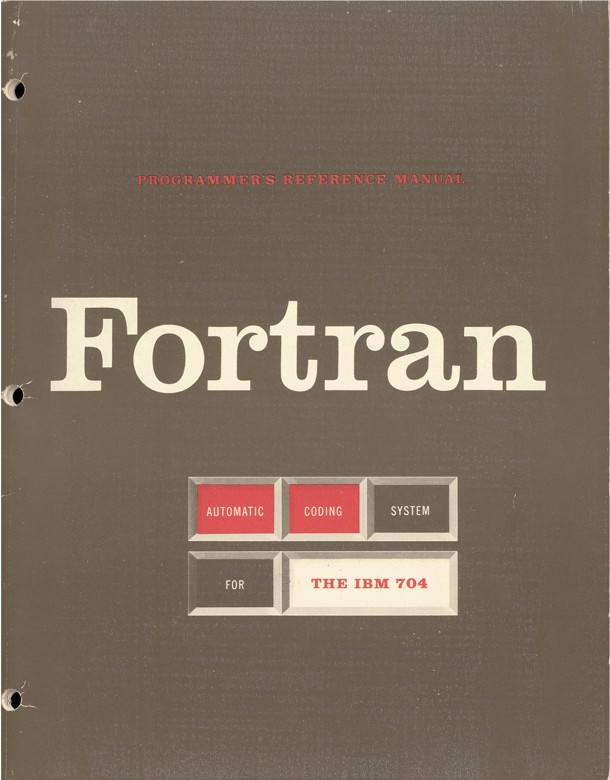
\includegraphics[scale=0.15]{pics/Fortran_acs_cover.jpeg}
    \end{column}
    \hfill
    \begin{column}{.76\textwidth}
      \begin{itemize}
        \item \normalsize{The User writes the source file:} \\
          \footnotesize{
          \code{program myprog} \\
          \code{  print *, 'Hello world'} \\
          \code{end program myprog}
          }
        \item \normalsize{A compiler parses source files and create
           binary object files:} \\
          \footnotesize{
          \code{gfortran -o -Wall -pedantic myprog myprog.f90}
          }
        \item \normalsize{Objects are linked with other objects or
           libraries to create executables:} \\
          \footnotesize{
          \code{0000000 457f 464c 0102 0001 0000 0000 0000 0000} \\
          \code{0000010 0003 003e 0001 0000 06f0 0000 0000 0000} \\
          \code{0000020 0040 0000 0000 0000 1a78 0000 0000 0000} \\
          \code{0000030 0000 0000 0040 0038 0009 0040 001d 001c} \\
          \code{0000040 0006 0000 0004 0000 0040 0000 0000 0000}
          }
      \end{itemize}
    \end{column}
  \end{columns}
\end{frame}


\end{document}

% vim: tabstop=8 expandtab shiftwidth=2 softtabstop=2 spell spelllang=en_uk
